\documentclass[11pt,a4paper]{article}
\usepackage[T1]{fontenc}
\usepackage[utf8]{inputenc}
\usepackage{lmodern}
\usepackage{microtype}
\usepackage[margin=22mm]{geometry}
\usepackage{amsmath}
\usepackage[table]{xcolor}
\usepackage{array,longtable,booktabs}
\usepackage{enumitem}
\usepackage{titlesec}
\usepackage{fancyhdr}
\usepackage[most]{tcolorbox}
\usepackage[hyphens]{url}
\usepackage{hyperref}
\usepackage{tikz}
\usetikzlibrary{arrows.meta,positioning,shapes.geometric,calc,fit,backgrounds}

\definecolor{ink}{HTML}{16202B}
\definecolor{accent}{HTML}{2458A6}
\definecolor{muted}{HTML}{4A5563}
\definecolor{rulec}{HTML}{CBD3DC}
\definecolor{shade}{HTML}{EEF2F6}
\definecolor{headbg}{HTML}{DCE6F2}
\definecolor{vfill}{HTML}{E9E8F7}\definecolor{vdraw}{HTML}{5B54B0}
\definecolor{sfill}{HTML}{E2F2EA}\definecolor{sdraw}{HTML}{2E8B63}
\definecolor{nfill}{HTML}{FBEBD2}\definecolor{ndraw}{HTML}{B5792A}
\definecolor{hfill}{HTML}{F8E4DD}\definecolor{hdraw}{HTML}{B5472E}

\hypersetup{pageanchor=false,colorlinks=true,linkcolor=accent,urlcolor=accent,citecolor=accent,
  pdftitle={CI+SIL x zz\_Workflow},pdfauthor={David Ramírez-Betancourt}}

\setlength{\parindent}{0pt}
\setlength{\parskip}{5pt}
\color{ink}

\titleformat{\section}{\Large\bfseries\color{accent}}{\thesection}{0.8em}{}[\vspace{-2pt}{\color{rulec}\titlerule}]
\titleformat{\subsection}{\large\bfseries\color{ink}}{\thesubsection}{0.8em}{}
\titlespacing*{\section}{0pt}{14pt}{6pt}

\pagestyle{fancy}
\fancyhf{}
\setlength{\headheight}{22pt}
\renewcommand{\headrulewidth}{0.4pt}
\renewcommand{\headrule}{\hbox to\headwidth{\color{rulec}\leaders\hrule height \headrulewidth\hfill}}
\fancyhead[L]{\small\color{muted}CI+SIL $\times$ zz\_Workflow}
\fancyhead[R]{\small\color{muted}v1.0 --- October 2026}
\fancyfoot[C]{\small\color{muted}\thepage}

\newtcolorbox{notebox}{enhanced,colback=shade,colframe=shade,boxrule=0pt,
  borderline west={2.5pt}{0pt}{accent},arc=0pt,left=8pt,right=6pt,top=5pt,bottom=5pt}

\tikzset{
  box/.style={draw=accent,fill=white,rounded corners=3pt,minimum height=10mm,
    minimum width=25mm,align=center,font=\footnotesize,text=ink,line width=0.6pt},
  acc/.style={box,fill=accent,draw=accent,text=white},
  mut/.style={box,draw=muted,fill=shade,text=ink},
  gap/.style={box,draw=rulec,fill=black!6,text=muted,dashed},
  gate/.style={diamond,align=center,draw=accent,fill=headbg,aspect=1.6,inner sep=1pt,
    font=\scriptsize,text=ink,line width=0.6pt},
  flow/.style={-{Stealth[length=3mm]},line width=0.7pt,color=accent},
  fb/.style={-{Stealth[length=3mm]},line width=0.6pt,color=muted,dashed},
  lbl/.style={font=\scriptsize,text=muted,align=center},
  vb/.style={box,fill=vfill,draw=vdraw,text=ink},
  sb/.style={box,fill=sfill,draw=sdraw,text=ink},
  nb/.style={box,fill=nfill,draw=ndraw,text=ink},
  hb/.style={box,fill=hfill,draw=hdraw,text=ink},
  node distance=8mm
}

\begin{document}

\begin{titlepage}
\thispagestyle{empty}
\vspace*{35mm}
{\color{accent}\rule{\textwidth}{1.2pt}}\\[8mm]
{\Huge\bfseries CI+SIL $\times$ zz\_Workflow\par}
\vspace{6mm}
{\Large\color{muted} Rationale for Coupling Continuous Integration with the LLM-Assisted Prototype Engine\par}
\vspace{8mm}
{\color{accent}\rule{\textwidth}{0.4pt}}
\vspace{20mm}

{\large\bfseries David Ramírez-Betancourt}\\[2mm]
{\large Universidad Nacional de Colombia --- GCPDS}\\[2mm]
{\large October 2026}
\vfill
\begin{notebox}\small
\textbf{Scope.} This note justifies, from the literature and from the project's own
context documents, why Continuous Integration with Software-in-the-Loop (CI+SIL) is the
first integration tier for the zz\_Workflow engine in the SDR FM sensor project.
\end{notebox}
\end{titlepage}

\section{Introduction}

The SDR FM sensor project uses an LLM-assisted workflow, zz\_Workflow, to produce verified
prototypes. The workflow constrains a language model inside four context-bounded stages
with human-gated transitions, and it ends in a prototype accompanied by recorded evidence.

What the project still lacks is a robust strategy for \emph{continuous} verification:
once a prototype exists, every later change to code, prompt, model, or context document
can silently invalidate the evidence that justified it. LLM-assisted systems make this
risk sharper, because the generator is probabilistic and its behaviour can shift without
any change to the source tree \cite{pith2026,mittal2026}.

This note compares the main validation methodologies against what zz\_Workflow already
produces, and argues for one coupling. \textbf{Thesis:} CI+SIL is the natural HIGH and
clean coupling. The regression suites that zz\_Workflow already requires are, in effect,
a CI harness, and replaying controlled I/Q in software needs no live RF. The coupling
preserves the engine's central rule that the model never approves its own work. It also
keeps claims honest: it delivers \emph{verification}, and it leaves live
\emph{validation} to downstream tiers.

Sections 2 to 4 give the foundation and the methodological landscape. Sections 5 and 6
cover AI-assisted hypothesis validation and the engine itself. Sections 7 to 9 analyse
the coupling, contrast it with the V-model in detail, and then refine it; Section 10
concludes.

\section{Foundation: Current AI Agents}

\textbf{Probabilistic, not deterministic.} LLM outputs vary even at nominal zero
temperature; the \emph{background temperature} induced by the inference stack makes
identical prompts yield different results \cite{pith2026}. Any workflow that assumes
repeatability must therefore measure it rather than assume it.

\textbf{A degradation ceiling.} Agent reliability decays roughly geometrically with the
number of sequential steps, with a practical ceiling near 16 steps \cite{mittal2026}. If
each step succeeds with probability $p$, a chain of $n$ steps succeeds with
$p^{n}$; the projected success at about 100 steps is only $\approx 0.24$. Long
autonomous chains are structurally fragile, which argues for short, bounded stages.

\textbf{Incentives favour hallucination.} Benchmarks that score accuracy alone reward
confident guessing over abstention, so models are trained to hallucinate
\cite{kalai2026}. Self-reported correctness is therefore weak evidence.

\textbf{Structure beats instructions.} Reliability gains come mainly from workflow
structure (typed interfaces, gates, retries, explicit state) rather than from longer
instructions \cite{nerd2026}. Likewise, \textbf{context engineering outranks prompt
engineering}: what the model sees at each step, and nothing more, is the controllable
variable \cite{anthropic2026}.

\textbf{Orchestration under constraints.} Surveyed agent systems orchestrate multiple
tools while managing state, cost, and safety constraints \cite{tooluse2026}. These are
the same constraints a verified-prototype pipeline must make explicit.

\section{Hardware Control via Tools}

An LLM only produces text. It reaches hardware through \emph{tools}, using function
calling and the Model Context Protocol (MCP) \cite{mcp2025,tooluse2026}. The resulting
closed loop is: agent $\to$ tool/MCP $\to$ actuator $\to$ sensor $\to$ feedback to the
agent.

\textbf{Two-level control.} The LLM plans at the slow level; a deterministic controller
executes the fast loop. The model never sits inside a real-time loop. \textbf{Physical
limits} declared in the tool's JSON Schema (ranges, units, enumerations) are the first
line of defence, since a call that violates the schema is rejected before it reaches
the device. Schema clarity also correlates with tool-call accuracy \cite{tooluse2026}.

Two human barriers complement this. \emph{Human-in-the-loop} (HITL) is an
\textbf{authorization} barrier: a person approves consequential actions. \emph{Hardware-in-the-loop}
(HIL) is a \textbf{validation} barrier: the control software is exercised against real or
emulated hardware \cite{opalrt2026}. Figure~\ref{fig:hw} shows both.

\begin{figure}[htbp]
\centering
\resizebox{\textwidth}{!}{%
\begin{tikzpicture}
  \node[acc] (llm) {LLM Agent\\(plans)};
  \node[gate,right=9mm of llm] (hitl) {HITL\\gate};
  \node[box,right=9mm of hitl] (mcp) {Tool / MCP\\(JSON Schema\\limits)};
  \node[mut,right=9mm of mcp] (act) {Actuator\\(deterministic\\controller)};
  \node[mut,right=9mm of act] (plant) {Plant /\\Hardware};
  \node[mut,below=14mm of plant] (sens) {Sensor};
  \node[box,below=14mm of mcp,minimum width=32mm] (hil) {HIL validation\\bench};
  \begin{scope}[on background layer]
    \node[fill=shade,draw=rulec,rounded corners=4pt,fit=(act)(plant)(sens),
      inner sep=4mm,label={[lbl]above:fast loop}] {};
  \end{scope}
  \draw[flow] (llm) -- (hitl);
  \draw[flow] (hitl) -- (mcp);
  \draw[flow] (mcp) -- (act);
  \draw[flow] (act) -- (plant);
  \draw[flow] (plant) -- (sens);
  \draw[fb] (sens.south) -- ++(0,-8mm) -| node[lbl,pos=0.25,above]{feedback} (llm.south);
  \draw[fb] (mcp.south) -- (hil.north);
  \draw[fb] (sens.west) -- node[lbl,above]{evidence} (hil.east);
  \node[lbl,above=1mm of hitl] {authorization};
\end{tikzpicture}}
\caption{Two-level agent--hardware control loop. The LLM plans; schema-bounded tools
and a deterministic controller act; HITL authorizes, HIL validates.}
\label{fig:hw}
\end{figure}

\section{Validation Methodologies Compared}

Five approaches are in common use: the \textbf{V-model} \cite{qmsdoc2026,sheridan2026b},
\textbf{CI+SIL with TDD}, \textbf{HIL benches} \cite{opalrt2026,sheridan2026a},
\textbf{LLM-as-judge with HITL} \cite{futureagi2026,bajestani2026}, and
\textbf{multi-criteria decision analysis (MCDA)} \cite{mcda2026}.

They share four principles: (i) verification is not validation; (ii) checks run from
cheap to expensive; (iii) an \emph{external oracle} decides; and (iv) humans act at
the extremes (framing and final decision). In short, \emph{nobody validates in one step;
you validate in layers}.

The need is empirical. Roughly 83\,\% of autonomous-research agents publish code, but
only 38\,\% provide reproducible artifacts \cite{verifgap2026}. And the key structural
rule is that the \textbf{oracle must not be the generator} \cite{judge2026}.

Figure~\ref{fig:phases} maps the layers to six phases and marks what zz\_Workflow
currently covers.

\begin{figure}[htbp]
\centering
\resizebox{\textwidth}{!}{%
\begin{tikzpicture}
  \node[acc,minimum width=20mm,font=\scriptsize] (p1) {1. Framing\\(G0)};
  \node[mut,right=9mm of p1] (p2) {2. Model\\(G1)};
  \node[acc,right=9mm of p2] (p3) {3. Software/CI\\(G2)};
  \node[gap,right=9mm of p3] (p4) {4. HIL bench\\(G3)};
  \node[acc,right=9mm of p4] (p5) {5. Judgment\\(G4)};
  \node[gap,right=9mm of p5] (p6) {6. Decision\\MCDA};
  \foreach \a/\b/\g in {p1/p2/G0,p2/p3/G1,p3/p4/G2,p4/p5/G3,p5/p6/G4}{
    \node[gate] (g\g) at ($(\a)!0.5!(\b)$) {\g};
    \draw[flow] (\a) -- (g\g); \draw[flow] (g\g) -- (\b);
  }
  \draw[fb] (p2.south) -- ++(0,-8mm) -| (p1.south);
  \draw[fb] (p3.south) -- ++(0,-12mm) -| (p2.south east);
  \draw[fb] (p4.south) -- ++(0,-8mm) -| (p3.south);
  \draw[fb] (p5.south) -- ++(0,-12mm) -| (p4.south east);
  \draw[fb] (p6.south) -- ++(0,-8mm) -| (p5.south);
  \node[acc,minimum width=4mm,minimum height=4mm,below=20mm of p2,label=right:{\footnotesize covered}] (l1) {};
  \node[mut,minimum width=4mm,minimum height=4mm,right=25mm of l1,label=right:{\footnotesize partial}] (l2) {};
  \node[gap,minimum width=4mm,minimum height=4mm,right=25mm of l2,label=right:{\footnotesize gap}] (l3) {};
\end{tikzpicture}}
\caption{Six-phase validation flow with gates G0--G4 and feedback paths. Phases 1, 3, 5
are covered by zz\_Workflow; phase 2 is partial; phases 4 and 6 are gaps.}
\label{fig:phases}
\end{figure}

\section{Validating Hypotheses with AI}

\textbf{Code is AI's strongest contribution.} The generate $\to$ execute $\to$ test
$\to$ repair loop turns model output into something an external executor can accept or
reject. Heinrichs et al.\ report hundreds of simulate--evaluate--modify iterations with an
LLM scripting CST, ADS, and KiCad \cite{heinrichs2026}.

\textbf{LLM-as-judge needs calibration.} Agreement with human raters should reach
Cohen's $\kappa \ge 0.6$ (and $\ge 0.8$ for strong agreement), with explicit controls
for position, verbosity, and self-preference bias \cite{futureagi2026,judge2026}.

\textbf{Simulation has a ceiling.} HIL enters when the restriction is hardware
\cite{opalrt2026}. HITL retains irreducible value: in the reported work, humans
detected geometry idealizations and routing inconsistencies that automated evaluation
missed \cite{bajestani2026,heinrichs2026}.

\begin{notebox}
``Validated in simulation'' does not mean ``validated.'' The claim must name the
environment in which the evidence was produced.
\end{notebox}

\section{The zz\_Workflow Engine}

zz\_Workflow has four context-bounded stages: \textbf{Ctx 00} (Problem Baseline),
\textbf{Ctx 01} (Requirements), \textbf{Ctx 02} (Architecture), and \textbf{Ctx 03}
(Implementation Contract). Transitions are human-gated: the model drafts but never
approves. The governing rule is:

\begin{notebox}
\emph{Acceptance is decided by pre-declared criteria applied to recorded
measurements, never by model judgement.}
\end{notebox}

The terminal output is a \textbf{Verified Prototype + Evidence}, which is explicitly
\emph{verification}, not validation. When a check fails, \textbf{R0--R3 defect routing}
returns the classified failure to the responsible stage.

Six governing artifacts support the engine. The most relevant here is \textbf{Artefact 3}:
the evaluation and benchmarking suites, which act as regression checks after \emph{any}
model, prompt, or context change. Figure~\ref{fig:zz} summarises the structure.

\begin{figure}[htbp]
\centering
\resizebox{\textwidth}{!}{%
\begin{tikzpicture}
  \node[acc,minimum width=48mm] (c0) {Ctx 00 --- Problem Baseline};
  \node[acc,minimum width=48mm,below=12mm of c0] (c1) {Ctx 01 --- Requirements};
  \node[acc,minimum width=48mm,below=12mm of c1] (c2) {Ctx 02 --- Architecture};
  \node[acc,minimum width=48mm,below=12mm of c2] (c3) {Ctx 03 --- Impl.\ Contract};
  \node[mut,minimum width=48mm,below=12mm of c3] (out) {Verified Prototype + Evidence};
  \foreach \a/\b in {c0/c1,c1/c2,c2/c3,c3/out}{
    \node[circle,draw=accent,fill=headbg,inner sep=1pt,font=\scriptsize\bfseries]
      (h\a) at ($(\a.south)!0.5!(\b.north)$) {H};
    \draw[flow] (\a) -- (h\a); \draw[flow] (h\a) -- (\b);
  }
  % R0-R3 feedback
  \draw[fb] (c1.east) -- ++(10mm,0) node[lbl,right]{R0} |- ([yshift=2mm]c0.east);
  \draw[fb] (c2.east) -- ++(18mm,0) node[lbl,right,xshift=0mm]{R1} |- ([yshift=-2mm]c0.east);
  \draw[fb] (c3.east) -- ++(26mm,0) node[lbl,right]{R2} |- (c1.east |- c1.south east);
  \draw[fb] (out.east) -- ++(34mm,0) node[lbl,right]{R3} |- (c2.east |- c2.south east);
  % artifacts sidebar
  \node[draw=rulec,fill=shade,rounded corners=3pt,align=left,font=\footnotesize,
    text width=48mm,anchor=north west,inner sep=4mm] (art) at ([xshift=62mm]c0.north east)
    {\textbf{Governing artifacts}\\[1mm]
     1. Problem baseline\\2. Requirements\\
     \textbf{3. Eval / benchmark suites}\\4. Contract\\5. Telemetry\\6. Evidence log};
\end{tikzpicture}}
\caption{zz\_Workflow stages with human gates (H), R0--R3 defect routing back to the
responsible stage, the six governing artifacts, and the terminal output.}
\label{fig:zz}
\end{figure}

\section{Coupling Analysis: Why CI+SIL}

Table~\ref{tab:coupling} rates each methodology by how directly it couples to what
zz\_Workflow already produces.

\begin{table}[htbp]
\centering
\caption{Coupling of each validation methodology with zz\_Workflow.}
\label{tab:coupling}
\small
\rowcolors{2}{white}{shade}
\begin{longtable}{@{}>{\bfseries\raggedright}p{30mm}>{\raggedright}p{28mm}>{\raggedright\arraybackslash}p{75mm}@{}}
\rowcolor{headbg}\textbf{Approach} & \textbf{Coupling} & \textbf{Reason}\\
\endhead
CI+SIL & HIGH / clean & Artefact 3 is already a regression harness; SIL replays I/Q without RF.\\
V\&V (V-model) & HIGH--MEDIUM & Matches the stage structure but adds heavy traceability overhead.\\
LLM-judge + HITL & MEDIUM & Useful for review, but conflicts with deterministic acceptance.\\
HIL bench & MEDIUM--LOW & Needs physical infrastructure not yet in the loop.\\
MCDA & LOW & Applies to multi-hypothesis choice, not to single-prototype verification.\\
\end{longtable}
\end{table}

\textbf{Artefact 3 already is the harness.} Coupling CI to it requires no new concept: the
suites run automatically instead of manually.

\textbf{The name is precise.} ``Verified'' $\ne$ ``validated'': the output claims
conformance to pre-declared criteria, not fitness in the field.

\textbf{Omitting LLM-as-judge for acceptance is a strength.} When the same component
proposes and evaluates, optimization pressure exploits evaluator weaknesses
\cite{judge2026}. The recipe is role separation plus deterministic gates, where
\emph{mechanical rejection beats LLM approval, never the reverse}.

Against the six phases of Figure~\ref{fig:phases}: phases 1, 3, 5 are \textbf{covered};
phase 2 is \textbf{partial}; phases 4 and 6 are \textbf{gaps}.

\section{V-model vs.\ CI+SIL}

The coupling table rates the V-model as a HIGH--MEDIUM alternative to CI+SIL. The two
are often read as rival paradigms, but they are not: \textbf{CI+SIL is the V-model's
right arm made continuous}. Understanding the relationship clarifies why CI+SIL is the
cleaner choice for zz\_Workflow while the V-model's structure is largely preserved.

\subsection{The classic V-model}

The V-model pairs a descending \emph{design/verification} arm with an ascending
\emph{testing/validation} arm \cite{qmsdoc2026,sheridan2026b}. Each left-hand level
(system requirements, system design, architecture design, module design) \emph{defines
the tests} for the right-hand level that mirrors it: requirements $\leftrightarrow$
acceptance, system design $\leftrightarrow$ system test, architecture
$\leftrightarrow$ integration, module design $\leftrightarrow$ unit test. The valley is
implementation. The dashed horizontals in Figure~\ref{fig:vclassic} are these
``defines-its-tests'' links. The model is strong on traceability and on separating
verification from validation, but in its classic form the entire right arm is a
\emph{single, late} pass: tests run once, after the full descent and ascent, and the
oracle arrives at the end.

\begin{figure}[htbp]
\centering
\resizebox{0.95\textwidth}{!}{%
\begin{tikzpicture}[x=16mm,y=13mm,every node/.style={font=\scriptsize}]
  % left descending design/verification arm
  \node[vb,minimum width=24mm] (req)  at (0,0)    {System\\requirements};
  \node[vb,minimum width=24mm] (dsys) at (1,-1.1) {System\\design};
  \node[vb,minimum width=24mm] (darq) at (2,-2.2) {Architecture\\design};
  \node[vb,minimum width=24mm] (dmod) at (3,-3.3) {Module\\design};
  \node[mut,minimum width=24mm](impl) at (4,-4.4) {Implementation\\(coding)};
  % right ascending testing/validation arm
  \node[sb,minimum width=24mm] (uni)  at (5,-3.3) {Unit\\tests};
  \node[sb,minimum width=24mm] (int)  at (6,-2.2) {Integration\\tests};
  \node[sb,minimum width=24mm] (sys)  at (7,-1.1) {System\\tests};
  \node[sb,minimum width=24mm] (acc)  at (8,0)    {Acceptance\\tests};
  % flow down and up
  \foreach \a/\b in {req/dsys,dsys/darq,darq/dmod,dmod/impl,impl/uni,uni/int,int/sys,sys/acc}{%
    \draw[flow] (\a) -- (\b);}
  % defines-its-tests dashed horizontals
  \draw[fb] (req)  -- (acc);
  \draw[fb] (dsys) -- (sys);
  \draw[fb] (darq) -- (int);
  \draw[fb] (dmod) -- (uni);
  % legend
  \node[vb,minimum width=3mm,minimum height=3mm] (lv) at (0,-5.4) {};
  \node[lbl,right=1mm of lv] (lvt) {Design / verification};
  \node[sb,minimum width=3mm,minimum height=3mm,right=12mm of lvt] (ls) {};
  \node[lbl,right=1mm of ls] (lst) {Testing / validation};
  \draw[fb] ([xshift=12mm]lst.east) -- ++(0.7,0) node[lbl,right,text=muted] {Defines its tests};
\end{tikzpicture}}
\caption{The classic software V-model. A descending design/verification arm (purple)
mirrors an ascending testing/validation arm (green); each left level \emph{defines the
tests} for the level facing it (dashed). Implementation sits at the valley, and the whole
right arm runs as a single late pass.}
\label{fig:vclassic}
\end{figure}

\subsection{Re-reading the right arm as CI+SIL}

CI+SIL keeps the same four test levels but changes \emph{when} and \emph{against what}
they run. Instead of one late pass, the levels execute automatically and continuously
against a software-modelled plant --- the SIL rung of the MIL$\to$SIL$\to$PIL$\to$HIL
ladder \cite{opalrt2026,sheridan2026a}:

\begin{itemize}[leftmargin=*,itemsep=1pt]
\item \textbf{Unit} (pure logic) runs \emph{on every commit}; \textbf{integration} (SIL)
  \emph{on every merge}; \textbf{system} (extended SIL) \emph{nightly}.
\item \textbf{Acceptance} stays at the apex as \textbf{HIL + real hardware} --- the one
  level that CI+SIL does \emph{not} absorb, and the shared downstream gap.
\item To run the lower arm without RF, CI+SIL adds a thin substitution layer (amber in
  Figure~\ref{fig:vmodel}): a \textbf{HAL} that abstracts the device behind an interface,
  a \textbf{Mock HAL} of driver stubs, and \textbf{synthetic data} (golden I/Q, injected
  error cases) that feed the mock. Purchased hardware sits behind the \emph{same} HAL,
  so the swap from mock to real device is transparent to the code under test.
\end{itemize}

\begin{figure}[htbp]
\centering
\resizebox{\textwidth}{!}{%
\begin{tikzpicture}[x=16mm,y=13mm,every node/.style={font=\scriptsize}]
  % left descending design/verification arm
  \node[vb,minimum width=24mm] (req) at (0,0)    {System\\requirements};
  \node[vb,minimum width=24mm] (dis) at (1,-1.1) {System\\design};
  \node[vb,minimum width=24mm] (arq) at (2,-2.2) {Architecture\\design};
  \node[vb,minimum width=24mm] (mod) at (3,-3.3) {Module\\design};
  \node[mut,minimum width=24mm] (cod) at (4,-4.4){Coding};
  % right ascending CI pipeline arm
  \node[sb,minimum width=24mm] (uni) at (5,-3.3) {Unit\\(pure logic)};
  \node[sb,minimum width=24mm] (int) at (6,-2.2) {Integration\\(SIL)};
  \node[sb,minimum width=24mm] (sys) at (7,-1.1) {System\\(extended SIL)};
  \node[hb,minimum width=24mm] (acc) at (8,0)    {Acceptance\\(HIL + real HW)};
  % design-arm flow
  \foreach \a/\b in {req/dis,dis/arq,arq/mod,mod/cod}{\draw[flow] (\a) -- (\b);}
  % CI pipeline flow with triggers
  \draw[flow] (cod) -- node[lbl,below,pos=0.55]{every commit} (uni);
  \draw[flow] (uni) -- node[lbl,right,pos=0.5]{every merge} (int);
  \draw[flow] (int) -- node[lbl,right,pos=0.5]{} (sys);
  \draw[flow] (sys) -- node[lbl,right,pos=0.5]{nightly} (acc);
  % defines-its-tests dashed horizontals
  \draw[fb] (req) -- node[lbl,above]{defines criteria} (acc);
  \draw[fb] (dis) -- node[lbl,above]{defines tests} (sys);
  \draw[fb] (arq) -- (int);
  \draw[fb] (mod) -- (uni);
  % substitution layer (new in CI+SIL)
  \node[nb,minimum width=24mm] (hal)  at (4,-5.8) {HAL\\(HW abstraction)};
  \node[nb,minimum width=24mm] (mock) at (6,-5.8) {Mock HAL\\(driver stubs)};
  \node[nb,minimum width=24mm] (dat)  at (6,-7.0) {Synthetic data\\(signals, errors)};
  \node[mut,minimum width=24mm] (hw)  at (1.4,-7.0){Purchased HW\\(sensor, SDR\dots)};
  \draw[flow] (cod) -- (hal);
  \draw[flow] (hal) -- (mock);
  \draw[flow] (dat) -- (mock);
  \draw[flow] (mock) -- (uni);
  \draw[flow] (hal) -- (hw);
  % CI feedback loop
  \draw[fb] (acc.east) -- ++(0.5,0) |- node[lbl,pos=0.25,right]{feedback} (dat.east);
  % legend
  \node[vb,minimum width=3mm,minimum height=3mm] (lv) at (0,-8.4) {};
  \node[lbl,right=1mm of lv] (lvt) {V-model original};
  \node[sb,minimum width=3mm,minimum height=3mm,right=10mm of lvt] (ls) {};
  \node[lbl,right=1mm of ls] (lst) {SIL tests (CI)};
  \node[nb,minimum width=3mm,minimum height=3mm,right=10mm of lst] (ln) {};
  \node[lbl,right=1mm of ln] (lnt) {New in CI+SIL};
  \node[hb,minimum width=3mm,minimum height=3mm,right=10mm of lnt] (lh) {};
  \node[lbl,right=1mm of lh] {HIL (lab)};
\end{tikzpicture}}
\caption{The V-model re-read as CI+SIL. The descending design arm (purple) is unchanged;
the ascending test arm (green) keeps the same four levels but runs continuously as SIL,
triggered on commit, merge, and nightly, against a Mock HAL fed by synthetic I/Q (amber).
Only acceptance stays at real hardware (red, HIL). The dashed horizontals are the
V-model's ``defines-its-tests'' links.}
\label{fig:vmodel}
\end{figure}

\subsection{Where they differ, and why CI+SIL wins here}

Table~\ref{tab:vcisil} contrasts the two along the dimensions that matter for an
LLM-assisted engine.

\begin{table}[htbp]
\centering
\caption{V-model versus CI+SIL on the dimensions relevant to zz\_Workflow.}
\label{tab:vcisil}
\small
\rowcolors{2}{white}{shade}
\begin{longtable}{@{}>{\bfseries\raggedright}p{30mm}>{\raggedright}p{52mm}>{\raggedright\arraybackslash}p{52mm}@{}}
\rowcolor{headbg}\textbf{Dimension} & \textbf{V-model} & \textbf{CI+SIL}\\
\endhead
Test cadence & One late pass after full descent/ascent. & Continuous: commit / merge / nightly.\\
Oracle timing & Arrives at the end. & Fires on every change, early.\\
Hardware need & Right arm tends to assume the target. & Lower arm runs on Mock HAL + synthetic I/Q; no RF.\\
Traceability & Explicit and heavy; its main cost. & Lighter; encoded in the suite and baseline.\\
Regression & Not intrinsic; re-runs are manual. & Intrinsic: every trigger re-runs the suite.\\
Fit to zz\_Workflow & Matches the gated, traceable stages, but adds ceremony. & Matches Artefact~3 (already a regression harness) and the trigger-on-any-change reality.\\
\end{longtable}
\end{table}

The V-model and CI+SIL agree on the two structural rules zz\_Workflow depends on: an
\emph{oracle distinct from the generator} and a clean \emph{verification} vs.\
\emph{validation} split, with live validation (HIL + field) left to the apex. They
differ on cadence and cost. The V-model's structure already resembles zz\_Workflow ---
gated stages, each defining its own acceptance --- which is why it scores HIGH--MEDIUM;
but its single late test pass and heavy traceability apparatus are a poor match for a
probabilistic generator whose behaviour can drift on \emph{any} model, prompt, or context
change. CI+SIL preserves the V-model's level structure while making the right arm
continuous and triggering on exactly those changes. It also demands no new concept from
the engine: Artefact~3 is already the regression harness the V-model's right arm would
have to build. The two are therefore not competitors but the same decomposition at two
cadences, and the continuous one fits the engine with less overhead.

\section{The Refined Coupling}

The coupling operates as follows (Figure~\ref{fig:coupling}).

\begin{itemize}[leftmargin=*,itemsep=1pt]
\item \textbf{Seed:} the evidence from the verified prototype (golden I/Q, Pd/Pfa curves)
  becomes the regression baseline.
\item \textbf{Version control:} code and the Ctx 03 contract live together as an
  executable specification.
\item \textbf{Trigger:} a change to the model, prompt, or any Ctx document, not only
  code commits. This is the natural CI adaptation for LLM-assisted systems.
\item \textbf{SIL:} replay of controlled I/Q (synthetic or recorded); no live RF.
\item \textbf{Regression:} Pd, Pfa, and latency compared against the evidence baseline.
\item \textbf{Acceptance gate:} deterministic, using the criteria from Ctx 01.
\item \textbf{Telemetry} (Artefact 5) records failure classes and points to the Ctx to
  revise. The R0--R3 routing is reused: CI states \emph{which} stage receives the defect.
\end{itemize}

Live-RF HIL remains a downstream gap.

\begin{figure}[htbp]
\centering
\resizebox{0.92\textwidth}{!}{%
\begin{tikzpicture}[node distance=7mm]
  \node[mut,minimum width=62mm] (vp) {Verified Prototype + Evidence};
  \node[box,minimum width=62mm,below=of vp] (vc) {Version Control\\(Code + Ctx 03 contract)};
  \node[acc,minimum width=62mm,below=of vc] (ci) {CI Pipeline\\(trigger: model / prompt / Ctx change)};
  \node[acc,minimum width=62mm,below=of ci] (sil) {SIL Replay\\(golden I/Q, no live RF)};
  \node[acc,minimum width=62mm,below=of sil] (reg) {Regression Check\\(Pd / Pfa / latency vs.\ baseline)};
  \node[acc,minimum width=62mm,below=of reg] (acc) {Acceptance Gate\\(deterministic, Ctx 01 criteria)};
  \node[box,below left=8mm and -8mm of acc,minimum width=24mm,draw=accent] (pass) {PASS};
  \node[box,below right=8mm and -8mm of acc,minimum width=24mm,draw=muted] (fail) {FAIL};
  \foreach \a/\b in {vp/vc,vc/ci,ci/sil,sil/reg,reg/acc}{\draw[flow] (\a) -- (\b);}
  \draw[flow] (acc.south) ++(-16mm,0) -- (pass.north);
  \draw[flow,color=muted] (acc.south) ++(16mm,0) -- (fail.north);
  \node[box,right=26mm of fail,minimum width=46mm,draw=muted,fill=shade] (route)
    {R0--R3 routing\\$\to$ responsible Ctx 00--03};
  \draw[flow,color=muted] (fail) -- (route);
  \draw[fb] (route.north) -- ++(0,0) |- (vc.east) node[lbl,pos=0.75,above]{revise, re-run};
  \begin{scope}[on background layer]
    \node[fill=shade,draw=rulec,dashed,rounded corners=4pt,fit=(ci)(sil)(reg)(acc),
      inner sep=3mm,xshift=-0mm] (tbox) {};
  \end{scope}
  \node[lbl,anchor=south west,xshift=2mm] at (tbox.north west) {};
  \node[box,left=10mm of sil,minimum width=26mm,draw=muted,fill=white] (tel)
    {Telemetry\\(Artefact 5)};
  \draw[fb] (tel.east) -- (tbox.west |- tel.east);
  \draw[fb] (fail.south) -- ++(0,-6mm) -| (tel.south);
\end{tikzpicture}}
\caption{CI+SIL coupled with zz\_Workflow. A model, prompt, or context change triggers
SIL replay and regression checks against the evidence baseline; a deterministic gate
decides, and failures are routed by R0--R3 to the responsible stage while telemetry
records the failure class.}
\label{fig:coupling}
\end{figure}

\section{Conclusion}

CI+SIL is the natural first integration tier for zz\_Workflow. The coupling is HIGH and
clean because Artefact 3 already is the regression harness: the evidence produced at
the end of the workflow seeds the baseline, and the Ctx 03 contract together with the
code serves as an executable specification under version control.

Deterministic gates preserve the principle that the model never approves its own work.
Triggering on model, prompt, or context changes, and not only on code commits, fits the
real failure modes of LLM-assisted systems. Reusing the R0--R3 routing lets CI say which
stage must revise the defect.

Two gaps remain downstream: an HIL bench for live RF validation, and MCDA for
selecting among multiple hypotheses. Keeping the distinction between \emph{verified}
and \emph{validated} makes the claims honest and the next steps tractable.

\begin{thebibliography}{99}\small
\setlength{\itemsep}{2pt}
\bibitem{tooluse2026} Harbin Institute of Technology \& Harvard, ``The Evolution of Tool Use in LLM Agents,'' arXiv:2603.22862, Mar.\ 2026.
\bibitem{kalai2026} A.\ T.\ Kalai \emph{et al.}, ``Evaluating LLMs for accuracy incentivizes hallucinations,'' \emph{Nature}, vol.\ 653, Apr.\ 2026.
\bibitem{mittal2026} Mittal, ``How Fast Do Agents Rot?,'' arXiv:2609.01660, Sep.\ 2026.
\bibitem{anthropic2026} Anthropic, ``Effective context engineering for AI agents,'' 2026.
\bibitem{nerd2026} Nerd Level Tech, ``AI Agent Reliability 2026: Structure Beats Instructions,'' 2026.
\bibitem{mcp2025} Model Context Protocol Specification, rev.\ 2025-06-18, \url{modelcontextprotocol.io}.
\bibitem{opalrt2026} OPAL-RT, ``Guide to HIL Testing,'' updated Sep.\ 2026.
\bibitem{verifgap2026} ``Autonomous Research Agents: Verification Gap,'' arXiv:2608.05179, Jun.\ 2026.
\bibitem{judge2026} ``LLM-as-a-Judge Is Not an Oracle,'' arXiv:2609.02246, Sep.\ 2026.
\bibitem{qmsdoc2026} QMSdoc, ``Traceability in V-Model,'' Jan.\ 2026.
\bibitem{sheridan2026a} Sheridan, ``Testing Embedded Systems 2026,'' Apr.\ 2026.
\bibitem{heinrichs2026} Heinrichs \emph{et al.}, ``From Prompt to Prototype: LLM-Driven RF Workflow,'' arXiv:2608.31006, Aug.\ 2026.
\bibitem{bajestani2026} Sadeqi Bajestani \emph{et al.}, ``HITL+LLM in smart manufacturing,'' \emph{J.\ Manufacturing Systems}, vol.\ 86, Jun.\ 2026.
\bibitem{futureagi2026} FutureAGI, ``LLM-as-a-Judge in 2026,'' updated Aug.\ 2026.
\bibitem{mcda2026} \emph{Sustainable Futures}, ``MCDA reliability,'' Jun.\ 2026.
\bibitem{sheridan2026b} Sheridan Tech, ``Design Validation vs Verification,'' Mar.\ 2026.
\bibitem{pith2026} Pith, ``Introducing Background Temperature,'' arXiv:2604.22411, 2026.
\end{thebibliography}

\end{document}
